\documentclass{article} % For LaTeX2e
\usepackage[usenames,dvipsnames,svgnames,table]{xcolor}
\usepackage{nips12submit_e,times}
\usepackage{amsmath}
\usepackage{amssymb}
\usepackage{url}
\usepackage{color}
\usepackage{graphicx}
%\documentstyle[nips12submit_09,times,art10]{article} % For LaTeX 2.09

\title{Structured Statistical Source Code Prediction\\
{\small CMU 10-701 (Machine Learning) - Final Project Report}}
\author{
  Cyrus Omar\\
  \texttt{comar@cs.cmu.edu}
  \And
  Salil Joshi\\
  \texttt{salilj@cs.cmu.edu}
  \And Fl\'avio Cruz\\
  \texttt{fmfernan@cs.cmu.edu}
}

\newcommand{\fix}{\marginpar{FIX}}
\newcommand{\new}{\marginpar{NEW}}

\usepackage{xypic}

\nipsfinalcopy % Uncomment for camera-ready version

\begin{document}


\maketitle

\section*{Introduction}
Programming languages are formal systems with rich syntactic and semantic structure. They are
also human systems, in that they are used extensively by people in patterned ways to express their
intent. Many tools are designed to help people write code more efficiently by predicting
the source code that a developer intends. For example, code completion systems for editors like Eclipse for Java display pop-up menus containing the members of to the class of the variable being manipulated. 

Typical code completion systems use only this sort of semantic
information about the language and the libraries being used, and do not incorporate data about how developers have written programs
in the past. Recent work by Hindle et al.~\cite{Hindle:2012:NS:2337223.2337322} demonstrated, however, that source code could be successfully predicted statistically
using a simple $n$-gram model that used a tokenized, rather than structural, representation of source code. 

Our project aims to unite the structured and statistical approaches to source code prediction.
That is, rather than using a tokenized representation of source code, we would like to do
statistical prediction on a more natural representation of source code: the typed syntax tree.  We can then condition our predictions using semantic information, specifically:
\begin{itemize}
\item the \emph{type}, denoted $\tau$, of the expression being predicted (e.g. \verb|int| or \verb|Color|)
\item the \emph{syntactic context}, denoted $\sigma$, in which the expression occurs (e.g. whether the expression is an argument of a function call, the guard of an \verb|if| statement, etc.)
\item the \emph{program context}, denoted $\Gamma$, in which the expression occurs (i.e. the set of variables paired with their types that are in scope at the location that the expression occurs.)
\end{itemize}

For example, if a user has entered the code \texttt{Planet destination = }, where \verb|Planet| is an enumeration containing \verb|Mercury|, \verb|Venus|, \verb|Earth|, etc. (but not \verb|Pluto|, of course), then we have that the expected type at the cursor is \verb|Planet|, the syntactic context is \emph{assignment}, and given a program context, our prediction space should only assign non-zero probabilities to:
\begin{itemize}
\item literal members of the \verb|Planet| enumeration (e.g. \verb|Planet.EARTH|)
\item variables and fields of type \verb|Planet| available from the program context
\item calls to methods available from the program context that have return type \texttt{Planet}\footnote{We can consider  operators like $+$ and $[]$ as methods of the built-in types in Java.}
\end{itemize}
To assign a probability to an expression, denoted $e$, we first determine how likely it is that the expression is of each of these three \emph{syntactic forms}, where syntactic forms are denoted $\phi$. For each form, we can then assign probabilities to particular expressions of that form according to some form-specific conditional distribution. This model can be understood as a graphical model, as shown in Figure \ref{graphicalmodel}, where the syntactic form is a latent variable. The conditional distributions for both the syntactic form and expression are learned using data gathered from analyses of prior code corpuses (smoothed using some suitable method in cases where enough information is not available).

\begin{figure}
    \begin{displaymath}
    \xymatrix{
      *+[F]{\color{ForestGreen}\txt{Type ($\tau$)}} \ar[dr] \ar[drr] & & \\
      & *+[F]{\color{black} \txt{Syntactic\\Form ($\phi$)}} \ar[r] & *+[F]{\color{cyan}\txt{Expression ($e$)}}  \\
      *+[F]{\color{ForestGreen}\txt{Syntactic\\Context ($\sigma$)}} \ar[ur] \ar[urr] & & *+[F]{\color{ForestGreen}\txt{Program\\Context ($\Gamma$)}} \ar[u]  
    }
    \end{displaymath}
\caption{A graphical model representing our approach. Green variables are always observed (we do not assign marginal distributions to them.) The syntactic form, $\phi$, is a latent variable, and the expression, $e$, is unknown. Note that the syntactic form is a function of the expression. \label{graphicalmodel}}
\end{figure}

In addition to the applications to code completion systems in code editors like Eclipse, more accurate source code prediction techniques could be useful for other programming tools. For example, programmers with severe physical impairments may benefit from predictive programming interfaces that allow them convey source code using devices more limited than a keyboard, incorporating the predictions to reduce the amount of information that needs to be conveyed explicitly by the user.

\section*{Related Work}
As mentioned above, work by Hindle et al. \cite{Hindle:2012:NS:2337223.2337322} showed that using a simple $n$-gram model of source code, represented as sequences of tokens, produced reasonably accurate predictions. This work (published this summer) suggested improving this model with structural and semantic information as future work. We have corresponded with the authors of this paper.

Work examining the ``uniqueness'' of software has found that source code can often be decomposed into commonly-seen motifs \cite{Gabel:2010:FSE}, further suggesting that prediction that uses structural information may be a particularly helpful approach in the domain of source code.

Code completion systems that use statistical information in a limited context, such as specifically for predicting which methods of a class will be called, have been proposed in the literature \cite{Bruch:2009:LEI:1595696.1595728,robbes_how_2008}. Other systems, such as Calcite \cite{mooty_calcite:_2010}, have produced contextually-relevant {\em code snippets} or examples drawn from a code corpus or web search, where more frequently encountered snippets are preferentially shown. These can all be construed as related, more specialized, variants of the approach we are taking in our project.

\section*{Method}
\newcommand{\asgn}{\textbf{assignment}}
\newcommand{\statement}{\textbf{statement}}
\newcommand{\argument}{\textbf{arg}}
\newcommand{\other}{\textbf{other}}

\newcommand{\lit}{\textbf{lit}}
\newcommand{\meth}{\textbf{meth}}
\newcommand{\var}{\textbf{var}}


\newcommand{\nm}[1]{\#\{#1\}}
\newcommand{\nmm}[1]{\#_M\{#1\}}

\subsection*{Probability Model}
      Our goal is to learn a model that allows us to produce $\mathbf{P}(e|\tau, \sigma, \Gamma)$. As we described informally above, we determine this probability by marginalizing over a latent variable that represents the \emph{syntactic form} of the expression, denoted $\phi$:
    $$P(e | \tau, \sigma, \Gamma) = \sum_{\phi \in \Phi} P(e | \phi, \tau, \sigma, \Gamma) P(\phi | \tau, \sigma)$$
As diagrammed in Figure \ref{graphicalmodel}, $\tau$ is the type of the expression, $\sigma \in \Sigma$ is the syntactic context, $\Gamma$ is the program context, and $\phi$ is the syntactic form. We consider syntactic contexts $\Sigma = \{\statement, \asgn, \argument, \other\}$ representing plain statements, assignments to variables, method arguments and a catch-all for other syntactic contexts (e.g. conditional and loop guards, return statements, etc.). We consider syntactic families $\Phi = \{\lit, \var, \meth\}$, representing literals (of built-in and enumeration types), variables and method calls, respectively. 

	  We use the following notation to represented quantities learned from training data below:
	  \begin{itemize}
	  \item $\nm{e, \tau, \phi, \sigma}$ represents the number of expressions in the training set constrained by the provided expression, type, syntactic form and program context (summing over any omitted categories.)
	  \item $\nmm{\tau_0.m, \sigma}$ represents the number of method calls to the method $\tau_0.m$ in the training set, constrained by the provided return type and program context (summing over any omitted categories.)
  	  \end{itemize}
  
  The conditional distribution for the syntactic forms is categorical, with the probability for each $\phi \in \Phi$ learned as:
  $$P(\phi | \tau, \sigma) = 
  \left\{
  	\begin{array}{ll}
	 	\frac{\nm{\phi,\tau, \sigma}}{\nm{\tau, \sigma}} & \nm{\tau, \sigma} \neq 0\\
		\frac{\nm{\phi, \sigma}}{\nm{\sigma}} & \mbox{o/w}
	\end{array}
	\right.
  $$
  
  That is, we use the empirical probability that that the expression has syntactic form $\phi$ given that the expression has type $\tau$ and is in syntactic context $\sigma$. If we have no data for type $\tau$ in that syntactic context, we marginalize over $\tau$.
  
  The conditional distribution for an expression $e$ given the syntactic form, if the actual syntactic form of $e$ is $\phi_e$, is broken down according to form as follows:
  
$$P(e | \phi, \tau, \sigma, \Gamma) =
\left\{
	\begin{array}{ll}
		P_{\lit}(e | \tau, \sigma, \Gamma) & \mbox{if } \phi = \phi_e = \lit\\
		P_{\var}(e | \tau, \sigma, \Gamma) & \mbox{if } \phi = \phi_e = \var\\
		P_{\meth}(e | \tau, \sigma, \Gamma) & \mbox{if } \phi = \phi_e = \meth\\
		0  & \mbox{if } \phi \neq \phi_e 
	\end{array}
\right.
$$
\paragraph{Literals}
For literals, we use the empirical probability of previously seen literals, assigning 0 probability to all others. Although ideally we would assign non-zero probability to unseen literals, not doing so simplifies our implementation considerably due to inadequacies in the Eclipse libraries used to query information about types (see below.)

$$P_{\lit}(e | \tau, \sigma, \Gamma) = 
\left\{
	\begin{array}{ll}
		\frac{\nm{e, \lit, \tau, \sigma}}{\nm{\lit, \tau, \sigma}} & \nm{\lit, \tau, \sigma} \neq 0\\
		0 & \mbox{o/w}
	\end{array}
\right.$$

\paragraph{Variables} Variables have highly limited lifespans, so there is little empirical data that we can gather about their usage within a novel context. Thus, we simply give all variables available in the program context equal probability. We denote the set of variables of type $\tau$ in $\Gamma$ as $V(\Gamma, \tau)$.

$$P_{\var}(e | \tau, \sigma, \Gamma) = 
\left\{
	\begin{array}{ll}
	\frac{1}{|V(\Gamma, \tau)|} & e : \tau \in \Gamma\\
	0 & \mbox{o/w}
	\end{array}
\right.$$
$$V(\Gamma, \tau) = \{ x | x : \tau \in \Gamma\}$$


\paragraph{Methods} For method invocations, we first assign a probability for the method itself, and then recursively assign probabilities to the argument expressions. The product of these probabilities is thus the probability of the expression as a whole.

$$P_{\meth}(e | \tau, \sigma, \Gamma) = 
\left\{
	\begin{array}{ll}
          P_m(\tau_o.m | \tau, \sigma, \Gamma) \prod_{i=1}^n P(e_i | \tau_i, \argument, \Gamma)  & \mathcal{M}(e, \tau, \Gamma)\mbox{ true} \\
	0 & \mbox{o/w}
	\end{array}
\right.$$

We must check that the expression is in fact a well-typed method invocation, which we can do using a type theoretic predicate:

$$\begin{array}{lll}
\mathcal{M}(e, \tau, \Gamma) & = & \exists o, m, n, e_1, \ldots, e_n, \tau_o, \tau_1, \ldots, \tau_n. (e \equiv o.m(e_1, \ldots, e_n))~\land\\
 & & 
\Gamma \vdash o : \tau_o~\land~\Gamma \vdash o.m : \tau_o \rightarrow (\tau_1 \rightarrow \cdots \rightarrow \tau_n) \rightarrow \tau~\land~\\
 & & \Gamma \vdash e_1 : \tau_1 \land \cdots \land \Gamma \vdash e_n : \tau_n
\end{array}$$

To calculate the probability of a method itself, we consider two cases. It may be a method that we have seen in the training set, in which case we use the empirical probability of that method in the provided syntactic context. It may also be a method that hasn't been seen in the training set. In this case, we give a uniform distribution over all such methods callable via a variable in the program context, which we denote $M(\Gamma, \tau)$. We weigh each of these two possibilities by approximating the likelihood that an unseen method is used by the empirical probability that a method was used only once in the training set, with a penalty factor $\eta$ in the denominator to ensure that some probability remains for unseen methods. 
\begin{align*}
P_m(\tau_o.m | \tau, \sigma, \Gamma) & =  P_{\text{unseen}}(\tau, \sigma)\frac{1}{|M(\Gamma, \tau)|} + 
P_{\text{seen}}(\tau, \sigma)\frac{\nmm{\tau_o.m, \sigma}}{\nm{\meth, \tau, \sigma}}\\
P_{\text{unseen}}(\tau, \sigma) & =  \frac{ |\{\tau_o.m | \nmm{\tau_o.m, \sigma} = 1\}|}{\nm{\meth, \tau, \sigma} + \eta}\\
P_{\text{seen}}(\tau, \sigma) & =  1 - P_{\text{unseen}}(\tau, \sigma)
\end{align*}

\subsection*{Implementation}
We used the Java programming language to perform experiments to analyze the effectiveness of our methodology. The ideas underlying our project are applicable to any statically typed programming language, but Java has some advantages that are are relevant to us. First, there are large Java code corpuses freely available. Second, there is prior work on predicting Java programs that we can use as a basis for evaluating our model \cite{QualitasCorpus:APSEC:2010}. Lastly, we can use the Eclipse IDE which gives us access to a powerful toolchain for working with Java programs.

We implemented our prediction model using the Eclipse Java Development Tools (JDT) library. This library provides facilities for parsing Java code, for traversing the AST to visit the relevant parts of the tree (such as method declarations or variable bindings etc.) and for retrieving type information.

To learn the parameters of our model, we determine the frequencies of each expression form, given its type and also it's syntactic context.
As above, the context can be either a \textit{variable declaration} (expression appears as the initializer of a variable), \textit{statement}, \textit{method argument} (expression is the argument of a method invocation) or \textit{other} (everything else).

We have implemented three code visitors to collect data about the three expression forms:

\begin{description}
   \item[Literal Visitor:] For primitive types such as integers, floats, doubles or strings we count the frequency of each literal in the code. For enumeration types (like \texttt{Planet}), we count the frequency of each element of the enumeration.

   \item[Variable Visitor:] For each type, we count the number of times a variable of this type was referenced in the code.

   \item[Method Visitor:] We group methods by the return type, so that we can count the number of times each method is used. We also collect data about all the declared methods.
\end{description}

For prediction, we make use of another visitor in order to go through all the expressions in the target file. To compute the probability of an expression $e$ at a certain point in the file, we determine the context $\sigma$ of $e$ and it's type $\tau$. We
then count the number of literals, variables and methods that we found during the collection phase with the same $\sigma$ and $\tau$. We can then do a case analysis on the form of $e$, consistent with the formulation given above:

\begin{itemize}
   \item For literals, we compute the relative frequency of all literals over all expressions forms, and multiply it by the relative frequency of the literal value in relation to all literals with the same type and context.
   \item For variables we also compute the relative frequency of variables over all expressions forms and divide this by the number of variables of the same type in the scope of $e$. To find all variables, we first find the method $m$ where $e$ is located and then traverse the AST of $m$ to locate all variables that appear before $e$ and have type $\tau$.
   \item For method invocations, we compute the relative frequency of methods over all expression forms and multiply it by the probability of a method being seen or not seen depending  on whether it was found during the data collection phase. If the method was not found before, we find all the methods with the same return type using the current scope to get this probability. Finally, we recursively multiply the previous result by the probability of each argument of the method $e$, to get the prediction of the whole expression.
\end{itemize}

\section*{Experiments}

%%Although the best method to test the quality of our models would be to perform an user study, we are a bit more limited in time and resources. Therefore, we used already available software code to automatically test our prediction facilities.

Our experiments makes use of freely available code corpuses listed in Qualitas Corpus~\cite{QualitasCorpus:APSEC:2010}.
Table~\ref{tab:projects} presents the projects we picked from the catalogue. We also show the number of files and
lines of code (LOC) of every project.

\setlength{\textfloatsep}{10pt}
\begin{table}[t]
\centering
\begin{tabular}{|l|c|c|l|}
\hline
\textbf{Project} & \textbf{\# Files} & \textbf{\# LOC} & \textbf{Description} \\
\hline
Ant & 1196 & 256039 & a software tool for automating software build processes \\
ANTLR & 394 & 66845 & a framework for implementing compilers \\
Art Of Illusion & 487 & 153645 & an open source 3D modelling and rendering studio \\
Axion & 237 & 42329 & a relational database system supporting SQL and JDBC \\
Batik & 1664 & 366506 & a library for manipulation of SVG files \\
FindBugs & 1149 & 207827 & a program that uses static analysis to look for bugs \\
%JFreeChart & 1005 & 321551 & a library for displaying professional charts \\
\hline
\end{tabular}
\caption{Software projects used in our experiments.}
\label{tab:projects}
\end{table}
For each project, we consider a subset of files for testing, the test set, and all the remaining files as the training set.
In our experiments we want to determine the probability of an observed expression $e$ according to our model (the prediction rate). Ideally, $P(e| \tau, \sigma, \Gamma)$ should be 1 since $e$ was the expression that was actually observed. Thus a high prediction rate implies an accurate model.

To reduce noise in our prediction rate, we use a ten-fold cross validation, where we select 10\% of the files at random as the test set and build our model by using the remaining 90\% of the files. For each file in the test set, we visit all the expressions (including sub-expressions) and compute the prediction rate. We then average the prediction rate of all expressions found to produce the prediction rate for that file. Finally, we average the prediction rate of all files to get a prediction rate for the current iteration of the cross validation procedure.

\subsection*{Baseline: The $n$-gram model}
For comparison with the state-of-the-art, we generated probabilities using an $n$-gram model~\cite{Hindle:2012:NS:2337223.2337322}, with $n = 3$ tokens. The $n$-grams were generated using a version of the CMU Language Modeling Toolkit and the probabilities were computed using a Python scripts as follows:

$$P(t_3, \ldots, t_n | t_1, t_2) = \prod_{i=3}^n P_{\text{ngram}}(t_i | t_{i-2}, t_{i-1})$$

In the above, the tokens $t_3, \ldots, t_n$ are the tokens from the expression, $e$, and $t_1$ and $t_2$ are the tokens immediately preceding $e$ in the program.

\subsection*{Results}
Figure \ref{results} compares the probabilities generated by both methods, showing that our method (SSCP) performed significantly better than the $n$-gram model across all projects.
\begin{figure}
\begin{centering}
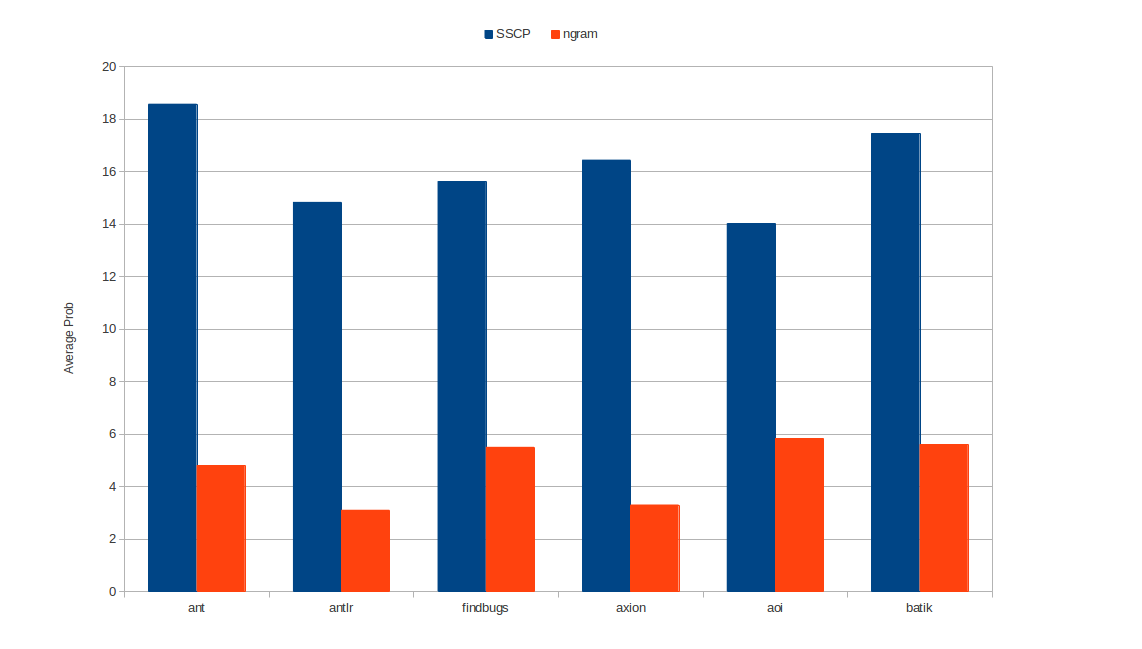
\includegraphics[scale=0.4]{overall.png}
\end{centering}
\caption{Results showing the average probability assigned to the actual expression for both the $n$-gram model (red) and our model (blue) for each of the six projects that we considered.\label{results}}
\end{figure}

\begin{figure}
\begin{centering}
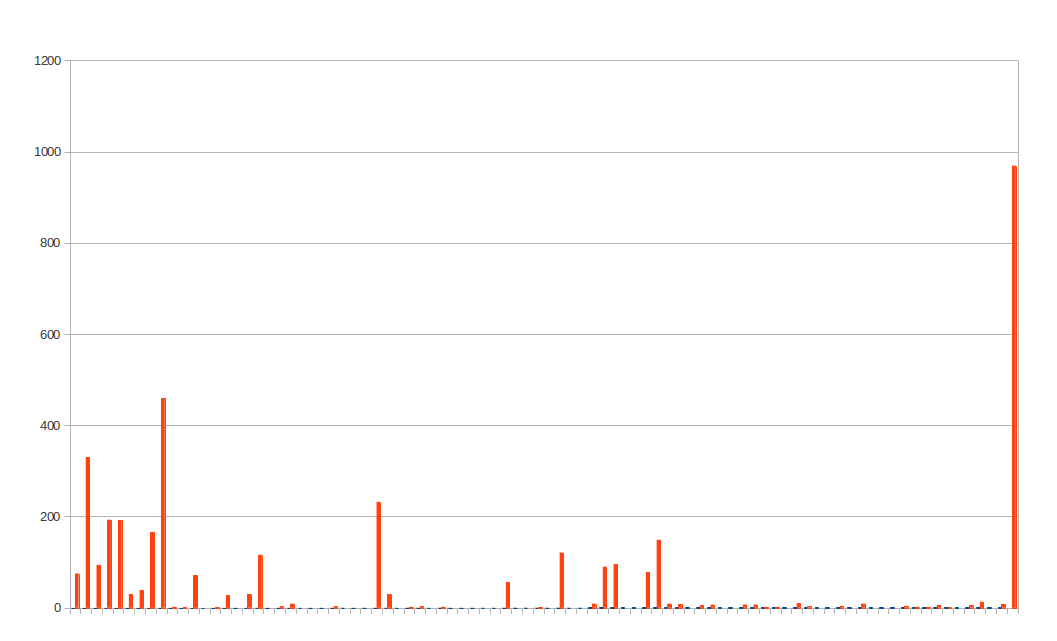
\includegraphics[scale=0.4]{ant.png}
\end{centering}
\caption{A histogram showing the distribution of probabilities assigned to expressions in the Ant project. The bucket for probabilities below 0.1 is omitted, as explained in the text. \label{hist}}
\end{figure}

We also analyzed the probabilities generated in a few of our runs to try and find areas where we can improve. Figure \ref{hist} shows a histogram of probabilities generated from one run on the ant project. The histogram is shown without the bucket of probabilities $< 0.01$ since there are so many of them. Analysis of our data revealed the following facts:

\begin{itemize}
  \item Our predictions are very good for variables. The average probability is high and even probabilities above 0.9 are not uncommon. This indicates that variables are used in predictable ways.
  \item Our predictions are very bad for \texttt{String}, \texttt{float}, \texttt{double}, and to a certain extent \texttt{int} literals. This is not surprising given our method, but these literals are so common that it would be useful to do something smarter in these cases. For example, for \texttt{int} literals we could imagine using an exponentially decreasing distribution that makes smaller numbers more probable, with added weights given to numbers we have seen before. For \texttt{Strings} we could use an underlying language model.
  \item Our predictions are also not very good when the expression is a method call. However this is only to be expected. In the case of a method call we are predicting a much larger expression, since we recursively predict the arguments and then multiply the probabilities. Our results improve dramatically if we consider only the \emph{name} of the method being called, which is all that would be required in an IDE code completion setting.
\end{itemize}

We also performed tests across projects i.e.\ we trained on one project and then calculated probabilities for expressions in a different project. The results are given in Table \ref{tab:cross}.

\begin{table}[h]
\centering
\begin{tabular}{|c|c|c|c|c|c|c|c|}
\hline
           & Ant   & ANTLR & AoI   & Axion & Batik & FindBugs \\
\hline
 Ant       & -     & 14.44 & 12.19 & 11.39 & 12.54 & 12.96    \\
ANTLR      & 14.04 & -     & 11.33 & 10.17 & 10.64 & 10.84    \\
AoI        & 18.94 & 17.3  & -     & 17.12 & 16.77 & 15.92    \\
Axion      & 15.93 & 14.74 & 12.08 & -     & 11.85 & 11.9     \\
Batik      & 18.71 & 17.35 & 15.11 & 13.84 & -     & 13.94    \\
FindBugs   & 17.23 & 16.00 & 14.16 & 12.97 & 13.18 & -        \\
\hline
\end{tabular}
\caption{Cross Project probabilities}
\label{tab:cross}
\end{table}

From this table we find that in most cases, within-project accuracy is higher than cross-project accuracy, which means that our method does learn facts that are local to the project (AoI is an exception to this rule, and we do not yet have a good explanation for its behavior).

Further, it seems possible that we can use cross-project prediction to learn interesting facts about the similarities between projects. For example, Ant is bad at predicting other projects, except for ANTLR. This is perhaps not a coincidence, because the Ant project has been designed to work well with ANTLR and has specific support for it. However, more analysis is required before we can be can determine whether cross-project accuracy is meaningful.


\section*{Conclusion}

We developed a prediction model for source code completion through the use of type and context information. Upon testing our model on open source code corpuses, we found that our model is several times more accurate than the current state of the art \cite{Hindle:2012:NS:2337223.2337322}, which indicates that using language semantics in addition to statistical information is useful.

There are several avenues for future work:
\begin{itemize}
  \item In the previous section we identified some shortcomings of our current model and discussed some possible improvements. We are actively working on these.
  \item We would like to use our model to provide better code completion in Eclipse, and as an aid to limited input devices.
  \item It seems possible that cross-project predictions can provide information about the similarities between projects. We would like to investigate this idea further.
\end{itemize}

\section*{Acknowledgments}

We are grateful to YoungSeok Yoon for providing example code for an Eclipse plug-in that we used to get started,  to Rachel Aurand for providing source code for the CMU Language Toolkit, and to Avinava Dubey for helpful feedback on the midway report.

\bibliography{midway}
\bibliographystyle{plain}

\end{document}
